\documentclass[10pt]{article}

\usepackage[letterpaper,margin=0.68in]{geometry}
\usepackage{enumitem}
\usepackage{tabularx}
\usepackage{booktabs}
\usepackage{xcolor}
\usepackage[hidelinks]{hyperref}
\usepackage{tikz}
\usetikzlibrary{arrows.meta,calc,positioning,shapes.geometric}

\definecolor{sourceblue}{HTML}{245B78}
\definecolor{sourcefill}{HTML}{E8F2F7}
\definecolor{leanblue}{HTML}{3056A3}
\definecolor{leanfill}{HTML}{E9EEFA}
\definecolor{auditgreen}{HTML}{24715A}
\definecolor{auditfill}{HTML}{E7F4EE}
\definecolor{closeorange}{HTML}{985B18}
\definecolor{closefill}{HTML}{FBF0DF}
\definecolor{releasegray}{HTML}{4A525A}
\definecolor{rulegray}{HTML}{D8DEE3}

\newcommand{\Lean}{Lean}
\newcommand{\file}[1]{\texttt{#1}}
\setlength{\parindent}{0pt}
\setlength{\parskip}{3pt}
\setlist[itemize]{leftmargin=1.25em,itemsep=1.4pt,topsep=2pt,parsep=0pt}
\setlist[enumerate]{leftmargin=1.45em,itemsep=2.5pt,topsep=2pt,parsep=0pt}
\pagestyle{plain}

\tikzset{
  flow/.style={-{Latex[length=2.2mm]},line width=0.8pt,draw=releasegray},
  evidence/.style={-{Latex[length=2mm]},line width=0.75pt,dashed,draw=auditgreen},
  auditnode/.style={draw,line width=0.8pt,rounded corners=2pt,align=center,
    minimum height=1.05cm,inner sep=4pt,font=\sffamily\scriptsize},
  source/.style={auditnode,draw=sourceblue,fill=sourcefill,text width=2.25cm},
  lean/.style={auditnode,draw=leanblue,fill=leanfill,text width=2.45cm},
  gate/.style={auditnode,draw=auditgreen,fill=auditfill,text width=2.35cm},
  closeout/.style={auditnode,draw=closeorange,fill=closefill,text width=2.35cm},
  release/.style={auditnode,draw=releasegray,fill=white,text width=2.35cm},
  tag/.style={font=\sffamily\bfseries\tiny,text=white,fill=releasegray,
    rounded corners=1pt,inner xsep=3pt,inner ysep=1.5pt}
}

\begin{document}

{\sffamily\bfseries\LARGE How a Paper Formalization Is Audited}\hfill
{\sffamily\small High-level procedure, August 2026}

\vspace{2pt}
\color{rulegray}\hrule\color{black}
\vspace{5pt}

\textbf{Purpose.}
The audit answers three different questions: (i) did we select the right claims
from the paper, (ii) do the elaborated \Lean{} declarations say the same thing,
and (iii) has \Lean{} proved those declarations without hidden mathematical
inputs?  A successful build answers only the third question for the statements
that were actually encoded.  Source fidelity and release certification require
their own evidence.

\begin{center}
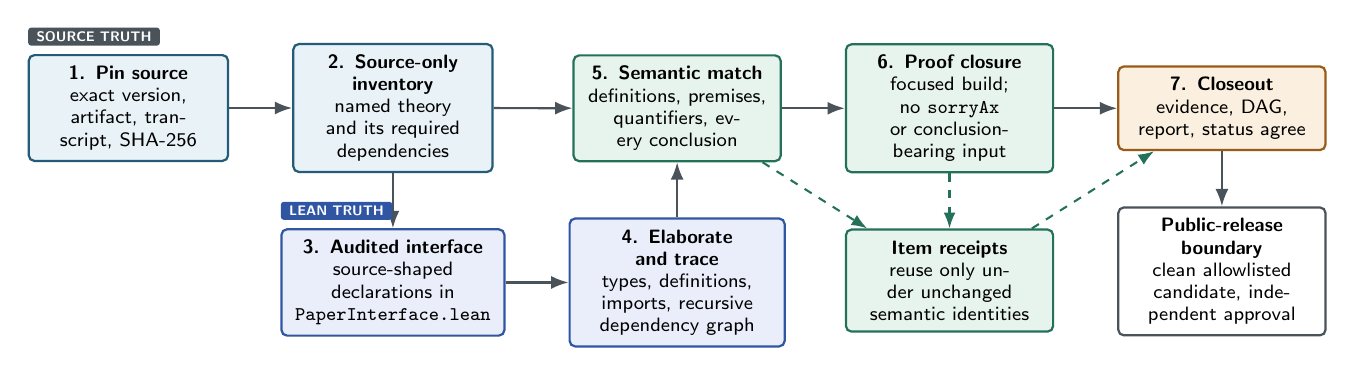
\begin{tikzpicture}[node distance=7mm and 8mm]
  \node[source] (pin) {\textbf{1. Pin source}\\exact version, artifact, transcript, SHA-256};
  \node[source,right=of pin] (inventory) {\textbf{2. Source-only inventory}\\named theory and its required dependencies};
  \node[lean,text width=2.55cm,below=of inventory] (interface) {\textbf{3. Audited interface}\\source-shaped declarations in \file{PaperInterface.lean}};
  \node[lean,right=of interface] (graph) {\textbf{4. Elaborate and trace}\\types, definitions, imports, recursive dependency graph};
  \node[gate,above=of graph] (semantic) {\textbf{5. Semantic match}\\definitions, premises, quantifiers, every conclusion};
  \node[gate,right=of semantic] (proof) {\textbf{6. Proof closure}\\focused build; no \file{sorryAx} or conclusion-bearing input};
  \node[closeout,right=of proof] (close) {\textbf{7. Closeout}\\evidence, DAG, report, status agree};
  \node[release,below=of close] (public) {\textbf{Public-release boundary}\\clean allowlisted candidate, independent approval};
  \node[gate,below=of proof] (receipts) {\textbf{Item receipts}\\reuse only under unchanged semantic identities};

  \draw[flow] (pin) -- (inventory);
  \draw[flow] (inventory) -- (interface);
  \draw[flow] (interface) -- (graph);
  \draw[flow] (inventory) -- (semantic);
  \draw[flow] (graph) -- (semantic);
  \draw[flow] (semantic) -- (proof);
  \draw[flow] (proof) -- (close);
  \draw[flow] (close) -- (public);
  \draw[evidence] (semantic) -- (receipts);
  \draw[evidence] (proof) -- (receipts);
  \draw[evidence] (receipts) -- (close);

  \node[tag,anchor=south west] at ($(pin.north west)+(0,1mm)$) {SOURCE TRUTH};
  \node[tag,anchor=south west,fill=leanblue] at ($(interface.north west)+(0,1mm)$) {LEAN TRUTH};
\end{tikzpicture}

{\footnotesize Solid arrows are required gates. Dashed arrows carry reusable evidence; they never bypass a gate.}
\end{center}

\textbf{The stages.}
\begin{enumerate}
  \item \textbf{Pin before interpreting.} Record the exact paper version and a
  byte-addressed, reviewable source artifact. A PDF may establish provenance,
  but normal inventory uses stable text or \TeX{} whose derivation is recorded.

  \item \textbf{Inventory from the source, not from the code.} Independently
  enumerate the normal surface: source-presented named definitions, models,
  assumptions, lemmas, propositions, theorems, corollaries, and theorem-like
  claims. Include an unlabelled item when a selected result depends on it.
  Figures, simulations, numerical examples, empirical claims, and standalone
  displays or algorithms are separate obligations only in explicit deep mode.

  \item \textbf{Write the review surface first.} Put the actual paper-facing
  definitions and theorem types, in paper order, in
  \file{PaperInterface.lean}. Proof plumbing belongs elsewhere. A private
  \file{by sorry} body may temporarily freeze an audited statement; it is a
  skeleton, never completion evidence.

  \item \textbf{Audit elaborated meaning.} \Lean{} elaborates the declarations,
  and the manifest records their name-independent proposition structure,
  reducible definitions, repository-local transitive dependencies, opaque
  imported terminals, and toolchain context. Recursive inspection follows
  record fields and aliases rather than trusting wrapper types.

  \item \textbf{Join source and \Lean{} item by item.} Coverage passes only when
  one complete pinned source presentation, one current elaborated declaration,
  and the premise/conclusion ledgers agree semantically. Names, numbering,
  routes, and similar prose are navigation aids, not evidence.

  \item \textbf{Close the mathematics.} Replace every temporary placeholder,
  build the complete paper target, and verify that the dependency closure has
  no \file{sorryAx}, axiom-like escape, or input record whose fields assume the
  advertised conclusion. A proof-body change reruns proof closure but need not
  invalidate an unchanged statement judgment.

\item \textbf{Close evidence before release.} Run the consolidated paper
  closeout, an independent source-first holistic audit, and the paper DAG/report
  checks. The canonical evidence, final report, and \file{status.json} must give
  one consistent account of assumptions, clarifications, boundaries, review, and
  mathematical status.
\end{enumerate}

\newpage

{\sffamily\bfseries\Large How the Audit Operation Runs}\hfill
{\sffamily\small Operational mechanics, not another mathematical gate}

\vspace{3pt}
The first diagram is the \emph{logical} audit flow: what must be established
about a paper. This diagram is the \emph{operational} flow: how the repository
creates one reproducible, current evidence record without two tools racing to
write it. These mechanics protect the audit; they do not themselves establish
that a source-to-\Lean{} bridge is mathematically correct.

\begin{center}
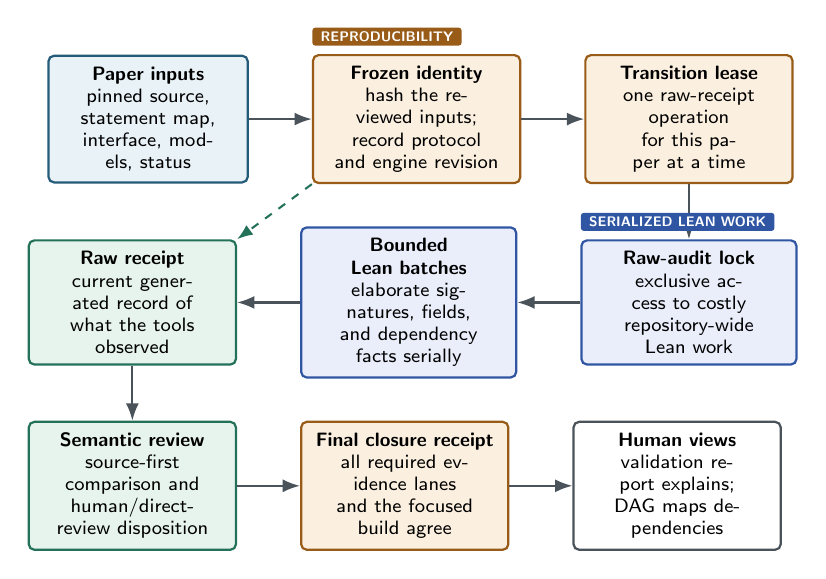
\begin{tikzpicture}[node distance=7mm and 8mm]
  \node[source] (inputs) {\textbf{Paper inputs}\\pinned source, statement map,\\interface, models, status};
  \node[closeout,right=of inputs] (freeze) {\textbf{Frozen identity}\\hash the reviewed inputs;\\record protocol and engine revision};
  \node[closeout,right=of freeze] (lease) {\textbf{Transition lease}\\one raw-receipt operation\\for this paper at a time};

  \node[lean,below=of lease] (lock) {\textbf{Raw-audit lock}\\exclusive access to costly\\repository-wide \Lean{} work};
  \node[lean,left=of lock] (batches) {\textbf{Bounded \Lean{} batches}\\elaborate signatures, fields,\\and dependency facts serially};
  \node[gate,left=of batches] (raw) {\textbf{Raw receipt}\\current generated record of\\what the tools observed};

  \node[gate,below=of raw] (review) {\textbf{Semantic review}\\source-first comparison and\\human/direct-review disposition};
  \node[closeout,right=of review] (final) {\textbf{Final closure receipt}\\all required evidence lanes\\and the focused build agree};
  \node[release,right=of final] (views) {\textbf{Human views}\\validation report explains;\\DAG maps dependencies};

  \draw[flow] (inputs.east) -- (freeze.west);
  \draw[flow] (freeze.east) -- (lease.west);
  \draw[flow] (lease.south) -- (lock.north);
  \draw[flow] (lock.west) -- (batches.east);
  \draw[flow] (batches.west) -- (raw.east);
  \draw[flow] (raw.south) -- (review.north);
  \draw[flow] (review.east) -- (final.west);
  \draw[flow] (final.east) -- (views.west);
  \draw[evidence] (freeze.south west) -- (raw.north east);

  \node[tag,anchor=south west,fill=closeorange] at ($(freeze.north west)+(0,1mm)$) {REPRODUCIBILITY};
  \node[tag,anchor=south west,fill=leanblue] at ($(lock.north west)+(0,1mm)$) {SERIALIZED LEAN WORK};
\end{tikzpicture}

{\footnotesize Solid arrows are operations that produce or check evidence. The dashed arrow records the exact frozen context that makes a raw receipt reusable.}
\end{center}

\textbf{What the operational layer does—and does not do.}
The audit engine
checks a frozen, named review surface according to the review protocol. The
lease, lock, and batches ensure that two executions cannot silently produce
incompatible records or exhaust the shared \Lean{} environment. They do not
choose the paper's claims, decide the intended mathematics, or substitute for
the source-first semantic review.

\textbf{Receipt hierarchy.}
The raw receipt is the detailed tool observation
for one frozen input identity. The final closure receipt names that raw evidence
and the required review lane, then records the paper-level disposition. The
validation report is a readable explanation of that decision; the DAG is a
readable map of the claims and their dependencies.

\newpage

{\sffamily\bfseries\Large Operational Glossary}\hfill
{\sffamily\small The vocabulary used by the implementation}

\vspace{5pt}
\begin{tabularx}{\textwidth}{@{}>{\bfseries\raggedright\arraybackslash}p{0.22\textwidth}
  >{\raggedright\arraybackslash}X@{}}
\toprule
Term & Meaning in this workflow \\
\midrule
Audit engine & The versioned implementation of the audit checks. Its code hash
and revision record make a run reproducible. It is an operational guard, not
mathematical evidence and not a verdict on the paper. \\
\addlinespace
Review protocol & The machine-readable policy defining audit scope and what a
current closeout must check. A protocol change can change obligations; an engine
change can instead be implementation-compatible. Both are recorded explicitly. \\
\addlinespace
Freeze / input identity & A snapshot of the precise source artifact, map,
review interface, source-model files, relevant configuration, and imported
\Lean{} closure. If one of these changes, a prior raw receipt is stale for the
new inputs rather than silently reused. \\
\addlinespace
Transition lease and lock & A lease prevents two closeout wrappers from trying
to preserve/reissue the same paper at once. The raw-audit lock separately
serializes expensive \Lean{} scans across the repository. Their heartbeats are
progress diagnostics, not evidence. \\
\addlinespace
\Lean{} batch & One bounded worker request, normally for a small exact set of
declarations. Batching controls memory and makes interruptions recoverable; it
does not split or weaken a mathematical review. \\
\addlinespace
Raw receipt & The generated, machine-readable source-record audit bound to the
frozen inputs. It reports elaboration and routing facts, including failures.
It is necessary evidence, but it is not the final human-facing validation. \\
\addlinespace
Final closure receipt & The one canonical machine-readable closeout record. It
binds the current raw evidence, required semantic/direct-review lane, focused
\Lean{} build, and status disposition. It replaces competing notions of a
``final report'' or an informal receipt. \\
\bottomrule
\end{tabularx}

\vspace{6pt}
\textbf{Why a fresh receipt is sometimes required.}
Changing a proof body can leave a
statement-level review current, while changing the source, map, interface,
source model, selected audit policy, or relevant imported \Lean{} content
changes the thing being audited. The workflow then records a new frozen
identity and reissues the raw receipt. A registered engine transition is also
placed in a new operational wave so that the record says exactly which audited
implementation produced it. This bookkeeping does \emph{not} erase prior
mathematical work or imply that the paper became false; it prevents an old
machine observation from being presented as if it described changed inputs.

\vspace{4pt}
\textbf{What to read.}
For a quick understanding of a paper, read the validation report and DAG. For
the exact closeout decision, read the final closure receipt it names. The raw
receipt and operation trace answer narrower questions such as ``what did the
tool see?'' and ``is a reissue still running?''; they are useful diagnostics,
not the primary narrative for a reader.

\newpage

{\sffamily\bfseries\Large What Must Match}\hfill
{\sffamily\small Semantic content, not identifiers}

\vspace{3pt}
\begin{tabularx}{\textwidth}{@{}>{\bfseries\raggedright\arraybackslash}p{0.19\textwidth}
  >{\raggedright\arraybackslash}X >{\raggedright\arraybackslash}p{0.31\textwidth}@{}}
\toprule
Dimension & Required agreement & Typical failure caught \\
\midrule
Source identity & Exact version, full byte-pinned presentation, source-only scope
classification, and stable locator. & Convenient excerpt omits a hypothesis;
map was built by looking at Lean names. \\
\addlinespace
Definitions and model & Objects, domains, encodings, normalization, tie-breaking,
state evolution, and relevant source conventions have the same mathematical
meaning. & A wrapper silently strengthens the model; a representation changes
the admissible inputs. \\
\addlinespace
Premises & Every source premise is represented; every visible or recursively
packed Lean premise is source-backed or proved from visible source premises by
an explicit checked bridge. & ``Certificate,'' record, or helper theorem
contains the desired conclusion as an assumption. \\
\addlinespace
Conclusions & Quantifiers, inequalities/equalities, cases, output guarantees,
and \emph{every} source conclusion atom are recovered. & Lean proves only one
direction, a restricted case, or existence without the advertised output. \\
\addlinespace
Algorithms and cost & When part of a selected named result, operational
semantics, termination, numeric model, and cost scope match as well as the final
mathematical relation. & A noncomputable existence wrapper is credited as a
polynomial-time algorithm. \\
\bottomrule
\end{tabularx}

\vspace{7pt}
\begin{minipage}[t]{0.49\textwidth}
{\sffamily\bfseries\large Reuse Without Re-auditing Everything}

Review receipts are cached \emph{per source item}. Reuse is allowed only when
all material identities remain unchanged:
\begin{itemize}
  \item source semantics and the byte-validated quote;
  \item elaborated, name-independent statement meaning;
  \item transitive semantic dependency graph and imported terminal artifacts;
  \item model/correction dispositions, protocol, validator, and toolchain
  context; and
  \item a unique current route to the same item.
\end{itemize}
A declaration, file, or map-key rename may be rebound only through a unique
semantic match. Missing, changed, or ambiguous identity fails closed. Thus a
small change reopens that item and affected dependents, not every unchanged
row. Reuse saves work; it is not independent evidence of correctness.
\end{minipage}\hfill
\begin{minipage}[t]{0.48\textwidth}
{\sffamily\bfseries\large Distinct Verdicts}

\begin{itemize}
  \item \textbf{Lean-closed:} all intended endpoints are proved under the
  displayed formal assumptions.
  \item \textbf{Source-audited:} source inventory, statements, premises,
  conclusions, definitions, and dependencies have current semantic evidence.
  \item \textbf{Human-reviewed:} a human has compared the pinned source with
  the complete review surface. LLM judgments are useful audit evidence, not a
  substitute for that review.
  \item \textbf{Release-certified:} source bytes are verified, required roles
  and approvals are recorded, and the exact public candidate passes the release
  boundary.
\end{itemize}
These axes are reported separately. A paper may be \Lean{}-closed while source
audit or release certification is still pending. Conversely, fresh audit
sidecars cannot make an open proof \emph{Formalized}.
\end{minipage}

\vspace{7pt}
\colorbox{closefill}{%
  \parbox{\dimexpr\textwidth-2\fboxsep\relax}{%
  \textbf{Public-release boundary.}
  Completed work is selected from the private incubator into a clean branch
  based on public \file{main}. A reviewed path allowlist, current canonical
  evidence, source-byte/license hygiene, the release guard, focused and
  integration builds, status synchronization, and explicit human approval bind
  the exact candidate. Private source artifacts, scratch work, historical audit
  snapshots, and unrelated papers are not carried into the public commit.}}

\vfill
{\footnotesize\color{releasegray}
Normative operational details live in
\file{config/formalization\_audit\_protocol.json}. The principal human guides
are \file{VALIDATION\_MODEL.md}, \file{PAPER\_COVERAGE\_AUDIT.md},
\file{INDEPENDENT\_AUDIT\_GUIDE.md}, and \file{PUBLIC\_RELEASE\_CHECKLIST.md}.}

\end{document}
